\documentclass[CMPE]{KGCOEReport}

\usepackage{float}
\usepackage{graphicx}
\usepackage{amsmath}
\newcommand{\classCode}{CMPE 160}  
\newcommand{\name}{Christopher Larson}
\newcommand{\LabSectionNum}{L3}
\newcommand{\LabInstructor}{Mr.\ Dominguez}	
\newcommand{\TAs}{TA Andrew Ramsey \\ TA Matthew Miller \\ TA Madeline Mooney}
\newcommand{\LectureSectionNum}{01}
\newcommand{\LectureInstructor}{Professor Beato}
\newcommand{\exerciseNumber}{04}
\newcommand{\exerciseDescription}{Combinational Logic Circuit Design Using Boolean Algrebra Simplification }
\newcommand{\dateDone}{7 February 2018}
\newcommand{\dateSubmitted}{14 February 2018}

\begin{document}
\maketitle

\section*{Abstract}
The objective of this exercise is to simplify Boolean algebraic expressions to a simplified expression and implement the expressions using a combinational logic circuit. Combination logic circuits provide control signals to device or perform mathematical operations. The logic gate designed in the exercise read a a single two-bit binary number, N= (N1,N0), and produced a single four-bit output, F=(W,X,Y,Z), which depends on the selection control signal, "C". If \textit{C} was "0" then the output value would be the square of N,  (F = $N^2$), and if \textit{C} was "1" then the output value would be fives times N, (F= 5N). The control signal, two-bit input and the four-bit output were recorded in a table and used to create the Boolean expressions used for the circuit. The physical cicuit performed the correct function that was theorized on the truth table.
\section*{Design Methodology}
The exercise used a two-bit binary number, N=(N1,N0) and a control signal to determine the output of the four-bit binary number shown in Table 1. The control signal determined whether the output was found using F= $N^2$ when \textit{C} was "0" and F = 5N when \textit{C} was "1".
\begin{table}[H]
	\centering
	\caption{Truth table for mathematical operations $N^2$ and 5N}
	\label{tab: Table 1}
	\begin{tabular}{|ccc||cccc|}
		\hline
		C & N1 & N0 & W & X & Y & Z\\ \hline
		0 & 0 & 0 & 0 & 0 & 0 & 0\\ \hline
		0 & 0 & 1 & 0 & 0 & 0 & 1\\ \hline
		0 & 1 & 0 & 0 & 1 & 0 & 0\\ \hline
		0 & 1 & 0 & 1 & 0 & 0 & 1\\ \hline
		1 & 0 & 0 & 0 & 0 & 0 & 0\\ \hline
		1 & 0 & 1 & 0 & 1 & 0 & 1\\ \hline
		1 & 1 & 0 & 1 & 0 & 1 & 0\\ \hline
		1 & 1 & 1 & 1 & 1 & 1 & 1\\
		\hline
	\end{tabular}
\end{table}

The outputs were then used to create sum of products Boolean expression, where each product term included all of the input variables. Using Boolean algebra properties the Boolean expressions were simplified so they could be implemented with the minimal parts from the lab kit. The simplification are shown below with the Boolean algebraic properties stated next to the step that they apply to.

\begin{equation} W(C,N1,N0) = \overline{C}N1N0 + CN1\overline{N0} + CN1N0  \end{equation} 
\begin{equation} (Distributivity) \overline{C}N1+N0 + CN1(\overline{N)} + N0) \end{equation}
\begin{equation} (Complements) \overline{C}N1+N0 + CN1 \end{equation}
\begin{equation} (Redundant Literal Rule) CN1 + N1N0 \end{equation}

\begin{equation} X(C,N1,N0) = \overline{C}N1\overline{N0} + C\overline{N1}N0+CN1N0 \end{equation} 
\begin{equation} (Distributivity) \overline{C}N1N0 + CN0(N1 + \overline{N1}) \end{equation}
\begin{equation} (Complements) \overline{C}N1N0 + CN0 \end{equation}

\begin{equation} Y(C,N1,N0) = CN1\overline{N0} + CN1N0 \end{equation}
\begin{equation} (Distributivity) CN1(\overline{N0} + N0) \end{equation}
\begin{equation} (Complements) CN1 \end{equation}

\begin{equation} Z(C,N1,N0) = \overline{C}\,\overline{N1}N0 + \overline{C}N1N0 + C\overline{N1}N0 + CN1N0 \end{equation}
\begin{equation} (Distributivity) N1N0(\overline{C} + C) + \overline{C }\,\overline{N1}N0 + C\overline{N1}N0 \end{equation}
\begin{equation} (Complements) N1N0 + \overline{C }\,\overline{N1}N0 + C\overline{N1}N0 \end{equation}
\begin{equation} (Distributivity) N1N0 + \overline{N1}N0(\overline{C} + C)	\end{equation}
\begin{equation} (Complements)	N1N0 + \overline{N1}N0 \end{equation}
\begin{equation} (Distributivity) N0(\overline{N1} + N1)	\end{equation}
\begin{equation} (Complements)	N0 \end{equation}

Using these simplified expressions, a circuit was designed using basic gates. These are limited to the gates that are in the lab kits, the gates used were Inverters, dual-input AND, triple-input NAND, and dual-input OR gates, as shown below in Figure 1.

\begin{figure}[H]
	\centering
	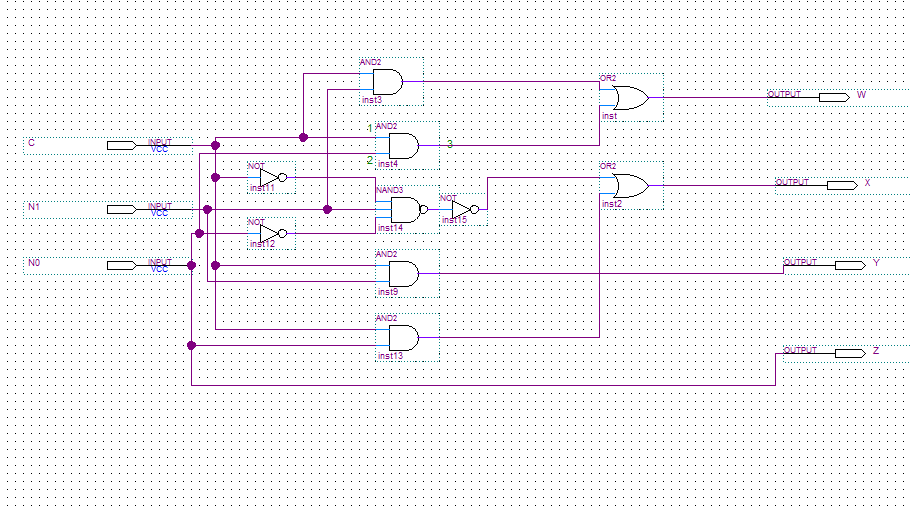
\includegraphics[width=0.65\textwidth]{QuartusL4}
	\caption{The schematic for the circuit built in Exercise Four}
	\label{fig: Figure 1}
\end{figure}

Using the circuit represented in Figure 1, the input and outputs were tested using four LEDs to test each of the outputs(W, X, Y, Z) and three switches for the inputs(C, N1, N0). A lit LED indicated that the gate was open and an unlit LED indicated that the gate was closed.

\section*{Results and Analysis}
In order to verify the correctness of Table 1, a simulation was created to generate a waveform that would verify the correctness of the schematic.

\begin{figure}[H]
	\centering
	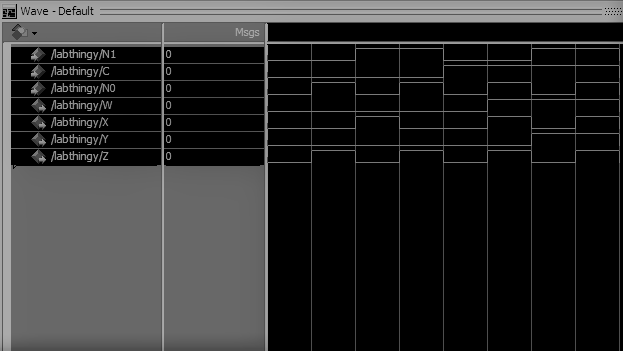
\includegraphics[width=0.65\textwidth]{ModelsimL4}
	\caption{The simulated waveform of the circuit built in Exercise Four}
	\label{fig: Figure 2}
\end{figure}

The waveform in Figure 2 matched the truth table in Figure 1 exactly and shows that the circuit design was correct. The test results from the breadboarded circuit are shown in Table 2.

\begin{table}[H]
	\centering
	\caption{Table of results for the LED test}
	\label{fig: Table 2}
	\begin{tabular}{|ccc||cccc|}
		\hline
		IN1 & IN2 & IN3 & LED1 & LED2 & LED3 & LED4\\ \hline
		0 & 0 & 0 & OFF & OFF & OFF & OFF\\ \hline
		0 & 0 & 1 & OFF & OFF & OFF & ON\\ \hline
		0 & 1 & 0 & OFF & ON & OFF & OFF\\ \hline
		0 & 1 & 1 & ON & OFF & OFF & ON\\ \hline
		1 & 0 & 0 & OFF & OFF & OFF & OFF\\ \hline
		1 & 0 & 1 & OFF & ON & OFF & ON\\ \hline
		1 & 1 & 0 & ON & OFF & ON & OFF\\ \hline
		1 & 1 & 0 & ON & OFF & ON & OFF\\ \hline
		\hline
	\end{tabular}
\end{table}

The results shown in Table 2 match the truth table shown in Table 1, where IN1 is input 1 and so on, and L1 is LED1 and so on. This shows that the circuit was constructed correctly.

\section*{Conclusion}
The use of Boolean algebraic properties is helpful in translating a truth table or a larger expression to a simplified and minimal expression that would be useful in a circuit. It is important to design and simulate the simplified expressions to ensure that the Boolean algebra was done correctly and still relevant. Once the expressions are simulated it is much simpler to create a functional circuit, and with the help of LEDs and switch can prove the expected results to be true. The exercise proved successful as the recorded results match the expected values.

\section*{Questions}
1. The equivalent gate count or EGC of the circuit is equal to the total number of dual-input gates required to implement the expression and in this case the answer is eight gates.

2.The chip count for basic gates of the circuit is the total number of chips required to implement the expression and in this case the answer is four chips.
\end{document}